\section{Formalization}
\label{sec:formalization}

\subsection{Intermediate Representation}
\label{subsec:ir}

A behavioral synthesis tool performs a number of compiler
and scheduling transformations (including pipelining). Certification of behavioral synthesis transformations thus requires a formalization of
the design representation manipulated by these
transformations. The formalization we use is {\em Clocked
  Control Data Flow Graph} (CCDFG)~\cite{rhcxy:atva-09}. 
Structurally, a CCDFG is a control and data flow graph augmented with a schedule. The control flow is broken into basic blocks. The instructions are grouped into microsteps which can be executed concurrently. A scheduling step represents a group of microsteps which can be executed in a single clock cycle. State of a CCDFG at a particular microstep is a list of all the variables of a CCDFG with their corresponding values.  The semantics of CCDFG require a formalization of the
underlying language used to represent the individual
instructions in a scheduling step.  The underlying language we use
is the LLVM language~\cite{llvm}. LLVM is a popular compiler
infrastructure for many behavioral synthesis tools~\cite{autoesl,xpilot} and includes an assembly language front-end.  We currently support
only a subset of LLVM operations which are required to handle all the designs we have
seen.  Instructions supported include assignment, load,
store, bounded arithmetic, bit vectors, arrays, and pointer
manipulation instructions.  Note that the reasoning involved 
in creating a pipelined CCDFG does not involve the exact 
syntax of any operation. We are merely concerned with a way 
to find the variables which are read and written at each step.
Increasing the operations database in our algorithm 
is expected to increase the time taken to prove certain primitives as much 
more analysis needs to be done.
However, it would not affect the logical reasoning of the primitives, the overall
algorithm and the proof.  
We define the syntax of each
type of statement by defining an ACL2 predicate.  For
example as shown in Figure~\ref{fig:syntax}, in our syntax, an {\em assignment statement} can be
expressed as a list of a variable and an
expression. An expression can further be of multiple types, %\eg, 
{\em load expression} (loading the value of a variable from memory), {\em add
expression} (addition of two variables), {\em xor expression} (xor of two variables)
etc., where each expression includes the operation applied to the
appropriate number of arguments. We provide semantics to these instructions through a
state-based operational formalization as is common with
ACL2~\cite{liu}. We define the notion of a CCDFG state, which includes
the states of the variables, memory, pointers, etc.  Then we
define the semantics of each instruction by specifying how
it changes the state.  Thus, for an assignment statement we
will have a function {\em execute-assignment} that specifies
the effect of executing the assignment statement on a CCDFG
state.

\begin{figure}
\begin{center}
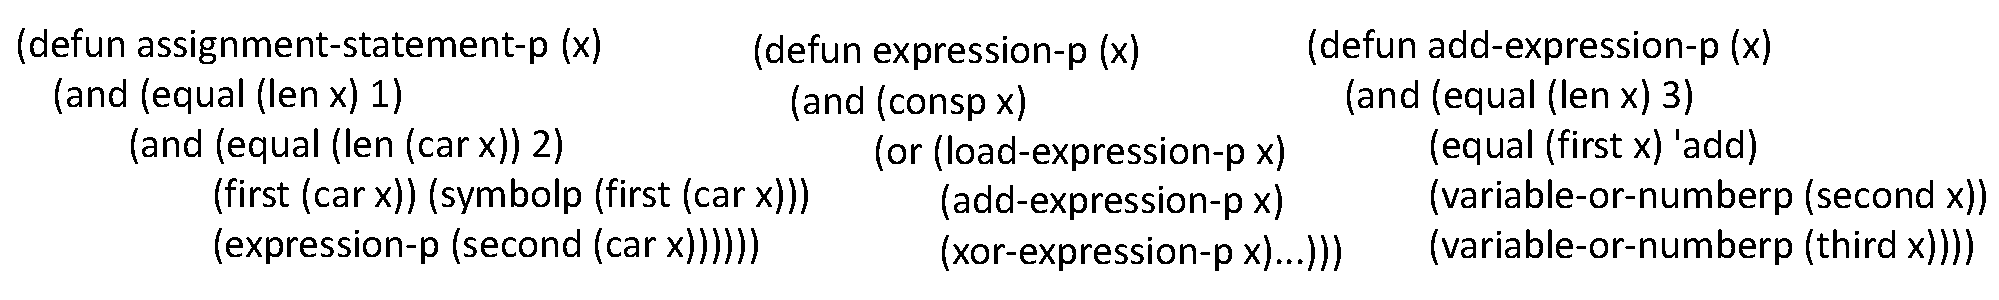
\includegraphics[width=4.5in]{fig-proposal/formalization}
\end{center}
\caption{ACL2 syntax}
\label{fig:syntax}
\end{figure}

%Defining the semantics of most supported statements is straightforward, with one exception.  The exception is the so-called ``$\phi$-construct'' available in LLVM~\cite{llvmphi}.  A $\phi$-construct is a list of $\phi$-statements.  A $\phi$-statement is $v := \phi [\sigma, bb1] [\tau, bb2]$, where $v$ is a variable, $\sigma$ and $\tau$ are expressions, and $bb1$ and $bb2$ are basic blocks: if it is reached from $bb1$ then it is the same as the assignment statement $v := \sigma$; if reached from $bb2$, it is the same as $v := \tau$; the meaning is undefined otherwise. The construct is complex since the effect of executing this statement on a CCDFG state $s$ depends not only on the state $s$ but also on how $s$ is reached by the control flow.
%Unfortunately, $\phi$-statements are required in loop designs --- they are used to evaluate the value of loop carried dependencies. Consequently, the complexity induced by this instruction cannot be avoided.

%\small
%\begin{verbatim}
%(defun phi-expression-p (x)
 % (and (consp x) (equal (len x) 1)
%       (consp (car x)) (> (len (car x)) 2)
 %      (equal (caar x) 'phi) (phi-l (cdr (car x)))))

%(defun phi-statement-p (x)
%  (and (consp x) (equal (len x) 2)
%       (symbolp (first x)) (first x)
%       (phi-expression-p (cdr x))))
%\end{verbatim}
%\normalsize

%Here {\tt phi-1} recognizes an expression of the form {\tt
%  ((E0 b) (E1 b-prime))} where {\tt E0} and {\tt E1} are
%expressions and {\tt b} and {\tt b-prime} are symbols
%representing basic blocks.  Thus in ACL2, the
%$\phi$-statement looks like {\tt (v (phi ((E0 b) (E1
%  b-prime))))}.  Finally, the execution semantics requires
%the additional parameter {\tt prev-bb} to track the previous
%basic block.

%% Comment: Function definition for execute-phi uses the functions
%%evaluate-val, replace-val and variables-of which are not
%%explained.

%\small
%\begin{verbatim}
%(defun choose (choices prev-bb)
% (if (or (equal (nth 1 (first choices)) prev-bb)
%          (equal (symbol-name (nth 1 (first choices))) prev-bb))
%      (nth 0 (first choices))
%    (nth 0 (second choices))))
    
%(defun evaluate-val (val bindings)
 % (if (symbolp val) 
 %     (cdr (assoc-equal val bindings)) 
 %   val))

%(defun execute-phi (stmt init-state prev-bb)
%  (let* ((expr (cdr stmt))
 %        (var (first stmt))
 %        (val (evaluate-val (choose (cdr (car expr)) prev-bb) 
 %                                  (car init-state))))
 %   (list (replace-var var val (variables-of init-state)) 
 %         (memory-of init-state) 
 %         (pointers-of init-state))))         
%\end{verbatim}
%\normalsize

%% Added
%The {\em init-state} represents the state of a CCDFG before executing $\phi$-statement. The function 
%{\em variables-of} is used to get a list of all the variables of {\em init-state} with their corresponding values. 
%{\em replace-var} replaces the values of the variable {var} to {val} in the list of those variables.

%.
%({\em e.g.}, AutoESL~\cite{autoesl}, xPilot~\cite{xpilot}).  
%We provide semantics to these instructions through a standard, state-based operational formalization~\cite{McCarthy}. It includes assignment, load, store, bounded arithmetic, bit ve XXX shows the formalization of a few instructions in ACL2.  As is standard with ACL2, the formalization specifies the effect  of execution of each instruction on the underlying abstract machine state based on the CCDFG representation.Executing a microstep ina CCDFG implies changing the current state of CCDFG based onmeaning of the instructions in the microstep and producing anew state. %Assigning meanings to most instructions is
%standard; one exception is the so-called ``$\phi$-construct''. A $\phi$-construct is a list of $\phi$-statements. A $\phi$-statement is $v := \phi [\sigma, X] [\tau, Y]$, where $v$ is a variable, $\sigma$
%and $\tau$ are expressions, and $X$ and $Y$ are
%scheduling steps: if it is reached from $X$ then it is the
%same as the assignment statement $v := \sigma$; if
%reached from $Y$, it is the same as $v := \tau$; the meaning is undefined otherwise. $\phi$-constructs are necessary due to the structure of the SSA (static single
%assignment) form of the LLVM code.

\subsection{Correctness of Loop Pipelining}
%A behavioral synthesis tool automatically generates a RTL design from an ESL design through a series of
%transformations. Pipelining a loop is a critical
%transformation in behavioral synthesis.
%\begin{enumerate}
%\item no nested loop;
%\item only one $Entry$ and one $Exit$ block; and
%\item no branching between the scheduling steps.
%\end{enumerate}

For the purposes of this paper, a {\em pipelinable loop} is a loop with the following restrictions~\cite{hrx:dac-12}: (1) no nested loop; 
(2) only one $Entry$ and one $Exit$ block; and (3) no branching between the scheduling steps.  
Our well-formed pipelinable loop has only one conditional branch and one unconditional branch. 
Unconditional branch is at the end of the loop dictating the back edge which enforces that the loop CCDFG is executed again from the first step. 
Conditional branch ensures that depending on the current value of the exit condition variable, a loop can exit if required. 
Other intermediate branches have already been handled by compiler and scheduling transformations prior to the pipelining transformation
so we need not consider them in our reasoning. There is one {\em $\phi$-construct}~\cite{llvmphi} in the first scheduling step which handles the value assigned
to loop carried variables depending on whether we are entering loop for the first time or not. These restrictions are not just meant to simplify the problem, but reflect the kind of loops that can be actually pipelined during behavioral
synthesis. For instance, synthesis tools typically require inner loops to have been fully unrolled (perhaps by a previous compiler
transformation) in order to pipeline the outer loop.

\begin{figure}[H]%[t!]
\begin{center}
\begin{tabular}{cc}
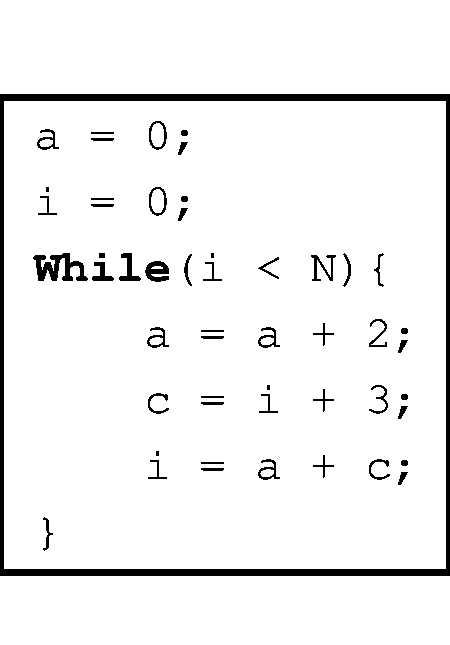
\includegraphics[height=1.5in]{fig-rpe/C-code}
& \hspace{2cm}
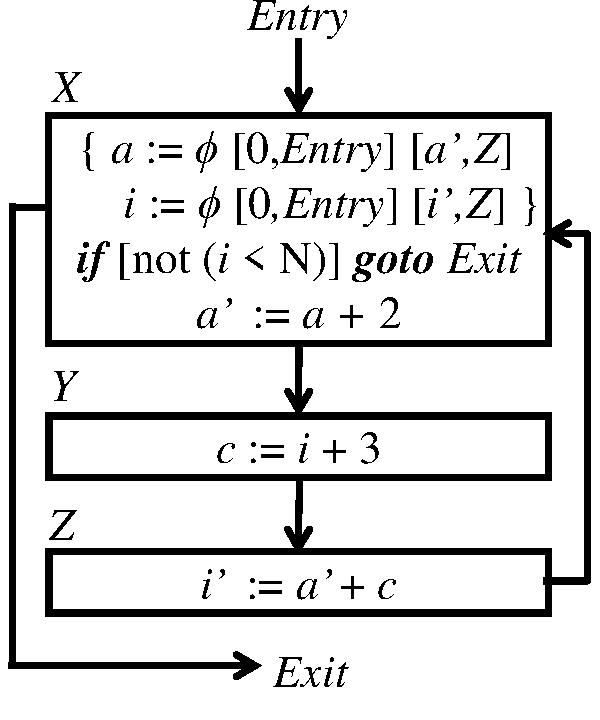
\includegraphics[height=1.5in]{fig-rpe/seq-ccdfg}
\\
(a) & \hspace{2cm} (b) 
\end{tabular}
\end{center}
\caption{(a) Loop in C (b) Loop CCDFG before pipelining.}
\label{fig:high-level-synthesis-1}
\end{figure}

Figure~\ref{fig:high-level-synthesis-1}(a) illustrates the C
code (ESL description) for a loop.  The C code does not have
a schedule or the concept of a clock cycle.
Figure~\ref{fig:high-level-synthesis-1}(b) shows CCDFG of the
sequential loop just before loop pipelining. The loop has
three scheduling steps: $X$, $Y$ and $Z$.  The scheduling
step before the loop is $Entry$ and after the loop is
$Exit$. The edges  in the CCDFG indicate the control flow.
Note that the sequential CCDFG has Static Single Assignment (SSA) structure
, as a result variable $a$ and $i$ are not assigned 
more than once and we require the quoted variables $a'$ and $i'$.

%% Since, reasoning about execution becomes difficult if we have to
%% always keep track of the previous scheduling step, we treat the first
%% iteration of the sequential CCDFG {\em seq-pre-loop} as a separate
%% iteration than the rest of the iterations {\em seq-loop}.  Infact, the
%% first step of our pipelining algorithm is to unroll the loop once and
%% replace $\phi$-construct by corresponding assignment statements based
%% on the previous scheduling steps.

%% \subsection{Correctness Statement}
%% \label{subsec:correctness-defn}

%% IMPORTANT : take a look again, if we want to keep all iterations same, we can start from k = 0

The main lemma involved in the correspondence proof between
the sequential and pipelined CCDFG can be paraphrased in English as follows. 

\begin{quote}
 If the pipeline generation succeeds without error,
 executing the pipelined CCDFG loop for $k$ iterations
 generates the same state of the relevant variables as
 executing the sequential CCDFG for some $k'$ iterations.
 The explicit value of $k'$ is given by the term {\tt (+ (-
   k 1) (ceil m pp-interval))}.
 \end{quote}

The theorem can be stated in ACL2 as follows.
%\footnote{The theorem mentioned in the paper does not contain all the hypotheses. Please refer to our proof scripts for final form of this theorem.}

\small
\begin{verbatim}
    
(defthm correctness-statement-key-lemma
    (implies (and (posp k)
                  (posp pp-interval)
                  (posp m)
                  (equal pp-ccdfg 
                     (superstep-construction pre loop pp-interval m))
                  (not (equal pp-ccdfg "error"))))
    (equal (in-order (get-real (run-ccdfg (first pp-ccdfg) 
                                         (second pp-ccdfg) 
                            	            (third pp-ccdfg) 
                            	            k init-state prev)))
              (in-order (run-ccdfg pre loop nil 
								               		                  (+ (- k 1) (ceil m pp-interval)) 
                                 		init-state prev)))))
\end{verbatim}
\normalsize

The theorem involves several ACL2 functions, \eg,
{\tt get-real}, \\ {\tt superstep-construction}, etc. 
For details, one can
  refer to our proof-scripts. 
%We do not
%discuss the detailed definitions of these functions in the
%paper, but they are available with the supporting ACL2
%script for this workshop.  
We provide a brief, informal
description of some of the critical functions in the theorem.
Two key functions that appear in the theorem above are {\tt
  superstep-construction} and {\tt run-ccdfg}. The function {\tt run-ccdfg} runs a CCDFG including a
pipelinable loop in three parts, first the prologue before the
loop, next the loop itself, and finally the epilogue past the
loop.
%\footnote{Of course one can have the standard function {\tt run} that executes the entire CCDFG rather than in parts.  However, for reasons that will be clear when we define the invariant, in our case it is easier to do most of the work with the execution in three parts and then assemble them into a final theorem about the CCDFG run in the end.}  
The function {\tt superstep-construction} combines the scheduling steps of successive iterations to create the ``scheduling supersteps'' of pipelined CCDFG.  If there are data-hazards and pipelined CCDFG cannot be generated as per
the pp-interval given, the function generates an ``error''.
Finally, the function {\tt get-real} removes from the
pipelined CCDFG state, all auxiliary variables introduced by
the pipeline generation algorithm itself, leaving only the
variables that correspond to the sequential
CCDFG,
%\footnote{The algorithm has to introduce new variables in order to eliminate hazards.  One consequence of this is that the new variables so introduced must not conflict with any variable subsequently used in the CCDFG.  Since we do not have a way to ensure generation of fresh variables, this constraint has to be imposed in the hypothesis.}  
and {\tt in-order} normalizes ``sorts'' the
components in a CCDFG state in a normal form so that the
sequential and pipelined CCDFG states can be compared with
{\tt equal}.
  %This function is defined as follows, where {\tt
  %prefix} determines the previous scheduling step of the
%iteration (required to resolve $\phi$-statements).

%\begin{verbatim}
%(defun run-ccdfg (pre loop post iterations init-state prev)
%  (let* ((state1 (run-block-set pre init-state nil prev))
 %        (state2 (run-blocks-iters loop state1 iterations (prefix loop)))
 %        (state3 (run-block-set post state2 nil (prefix post)))
 %   state3))
%\end{verbatim}




%\smallskip
%\noindent {\textbf {Correctness Statement:}}
%Let $L$ be a loop in CCDFG $C$, and let $L_{\alpha}$ be the
%pipelined implementation generated by a pipeline algorithm using
%pipeline parameters $\alpha$.  Let $V$ be the set of
%variables in $L$, and $U$ be the set of all
%variables in $C$.  Suppose we execute $L$ and $L_{\alpha}$
%from CCDFG states $s$ and $s'$ respectively, such that for
%each variable $v\in V$, the value of $v$ in $s$ is the same
%as that in $s'$, and suppose that the state on termination
%are $f$ and $f'$ respectively.  Then (1)~for any $v\in V$,
%the value of $v$ in $f$ is the same as that in $f'$, and
%(2)~for any $v\in(U\backslash V)$, the value of $v$ in $f'$
%is the same as that in $s'$.

%\medskip
%\noindent
%{\em Remark:} Condition (2)
%ensures that variables in $C$ that are not part of the loop
%are not affected by $L_{\alpha}$.  The value of any new
%variables introduced by the algorithm in $f'$ are irrelevant since they are not accessed
%subsequently.



%\subsection{Loop Pipelining Transformation}
%\label{subsec:loop-pipelining-trans}
%For our purposes, {\em pipelinable loop} is a loop with the following additional restrictions~\cite{hrx:dac-12}:
%\begin{enumerate}
%\item no nested loop;
%\item only one $Entry$ and one $Exit$ block; and
%\item no branching between the scheduling steps.
%\end{enumerate}
%These restrictions reflect the kind of loops that can be actually pipelined during behavioral synthesis. For instance, synthesis tools typically require inner loops to have been fully unrolled  in order to pipeline the outer loop.


%\begin{figure}[H]%[t!]
%\begin{center}
%\begin{tabular}{cc}
%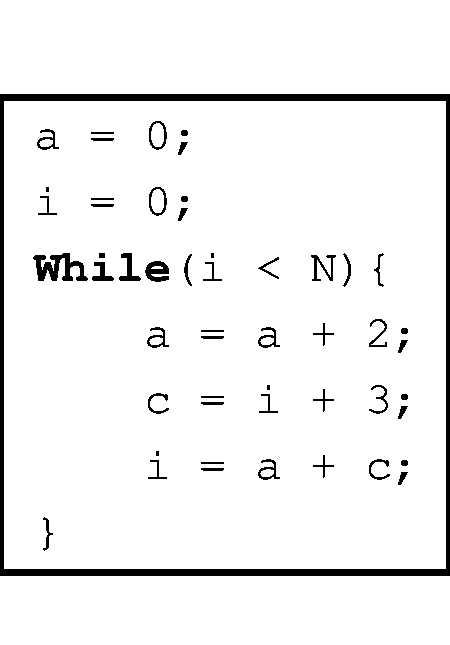
\includegraphics[height=1.5in]{fig-rpe/C-code}
%& \hspace{2cm}
%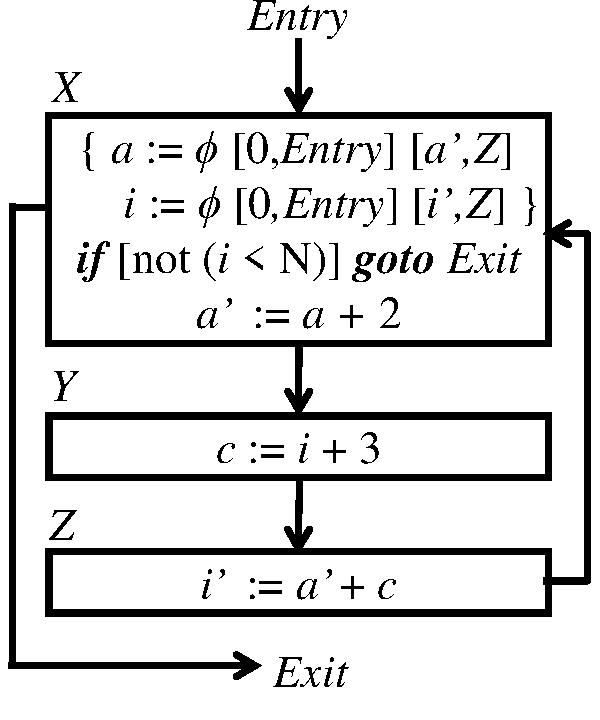
\includegraphics[height=1.5in]{fig-rpe/seq-ccdfg}
%\\
%(a) & \hspace{2cm} (b) 
%\end{tabular}
%\end{center}
%\caption{(a) Loop in C (b) Loop CCDFG before pipelining.}
%\label{fig:high-level-synthesis}
%\end{figure}

%Figure~\ref{fig:high-level-synthesis}(a) illustrates the C code for a loop at the beginning of the synthesis process. The C code does not have a schedule or the concept of a clock cycle. Figure~\ref{fig:high-level-synthesis}(b) shows CCDFG of the sequential loop just before loop pipelining. The loop has three scheduling steps: $X$, $Y$ and $Z$.  The scheduling step before the loop is $Entry$ and after the loop is $Exit$. Since, there are three scheduling steps in the loop, one iteration can be executed in three clock cycles.

%\begin{figure}
%\begin{center}
%\begin{tabular}{cc}
%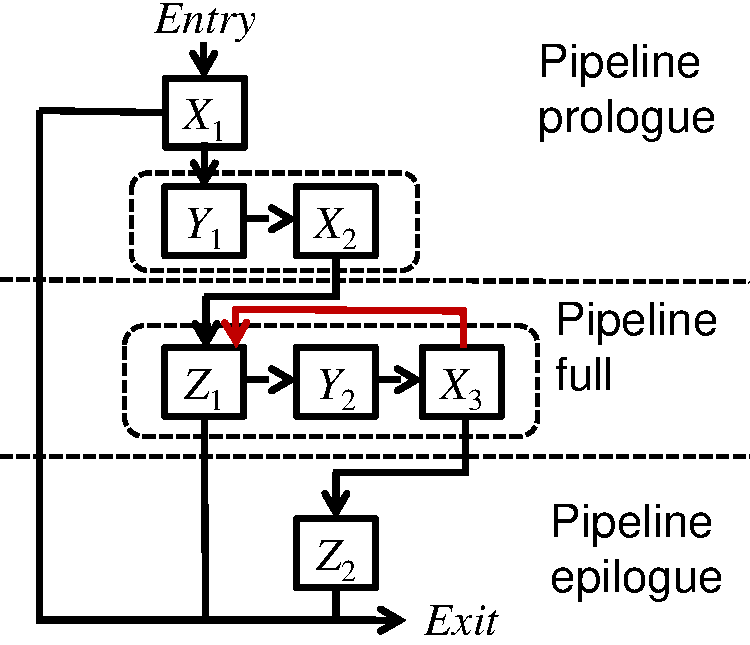
\includegraphics[height=1.5in]{fig-rpe/pipelined_ccdfg}
%& \hspace{0.5cm}
%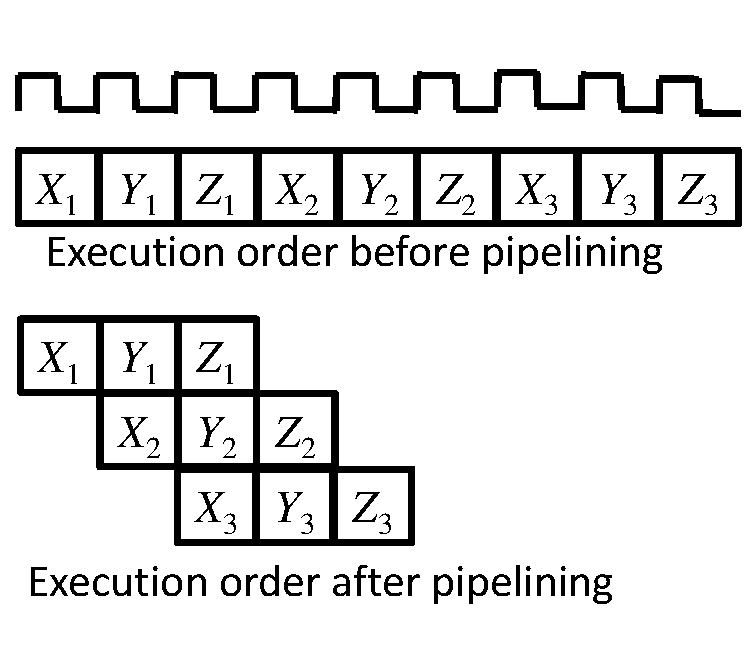
\includegraphics[height=1.5in]{fig-rpe/pp-clock-cycles}
%\end{tabular}
%\end{center}
%\caption{Pipelined CCDFG. The horizontal arrows indicate data forwarding.}
%\label{fig:pp-ccdfg}
%\end{figure}

%:Behavioral synthesis tools use complicated heuristics and aggressive scheduling strategies to find an optimized pipeline interval (clock cycles after which a new iteration can be started such that there are no data hazards). Figure~\ref{fig:pp-ccdfg} shows the pipelined CCDFG with a pipeline interval equal to one. The new scheduling steps in the pipelined CCDFG created by combining scheduling steps from different iterations of the sequential CCDFG are called scheduling supersteps. Observe that the three iterations of the pipelined loop take five clock cycles as opposed to nine clock cycles in the sequential loop. Loop pipelining reduces the number of clock cycles required to execute the loop, hence this transformation is used by synthesis tools to increase throughput and reduce latency.  

%\subsection{Correctness of Pipelined CCDFG}
%\label{subsec:correctness-defn}

%Correctness of loop pipelining can be informally stated as below.

%\begin{quote}
%Let $L$ be a loop in CCDFG $C$, and let $L_{\alpha}$ be the pipelined loop CCDFG. Let $V$ be the set of variables mentioned in $L$, and $U$ be the set of all variables in $C$.  Suppose we execute $L$ and $L_{\alpha}$ from CCDFG states $s$ and $s'$ respectively, such that for each variable $v\in V$, the value of $v$ in $s$ is the same as that in $s'$, and suppose that the state on termination are $f$ and $f'$ respectively.  Then (1)~for any $v\in V$, the value of $v$ in $f$ is the same as that in $f'$, and (2)~for any $v\in(U\backslash V)$, the value of $v$ in $f'$ is the same as that in $s'$.
%\end{quote}
%\noindent
%{\em Remark:} Condition (2) is the {\em frame rule} which ensures that variables in $C$ that are not part of the loop are not affected by $L_{\alpha}$.

